\documentclass{article}
\usepackage[]{hyperref}
\usepackage[utf8]{inputenc}
\usepackage{authblk}
\usepackage{braket}
\usepackage{listings}
\usepackage{graphicx}
\usepackage[]{amsmath}
\usepackage[]{amsfonts}
\usepackage[]{amssymb}
\usepackage{biblatex}
\usepackage{amsthm}
\newtheorem{theorem}{Theorem}
\title{Example file for easy creation of a LaTeX file from Markdown}
\author[1]{clemrouxx }
\affil[1]{ETH Zürich}
\date{Today's date !!!}
\addbibresource{bibliography.bib}

\begin{document}
\maketitle
\begin{abstract}

This paper show a fairly minimal example of file that can be transcompiled from Markdown to LaTeX and eventually to PDF, in the general style of a preprint. Although the style can be personalized using imported or custom LaTeX packages, this project has the advantage of implementing ways to label, reference and cite inside of the markdown file, in addition to other features, such as writing the abstract just as a modified quote (a "callout" in Obsidian terms).
\end{abstract}
\begin{maincontent}

\section{Goals}

We try to provide a markdown to LaTeX program oriented towards scientific articles or preprints. We give ourselves the following guidelines :
\begin{itemize}
\item 
The user should have as little LaTeX code to write as possible

\item 
But : it should still be feasible to customize the output style to a certain extent

\item 
The Markdown file should still be readable

\item 
The user shouldn't have to memorize some too specific syntax

\item 
Ideally, it should look nice in Obsidian, and be consistant with its parsing

\end{itemize}

\section{Examples}

\subsection{Modification of basic features}

In our program, all inserted images will be transformed into Figures. As such, the program expects a label (just after the image, preceded with a caret "\^{}"), and a caption (A paragraph of text just after the label and a line break). The usual prefix "fig:" for the label will be added automatically.


\begin{figure}
    \centering
    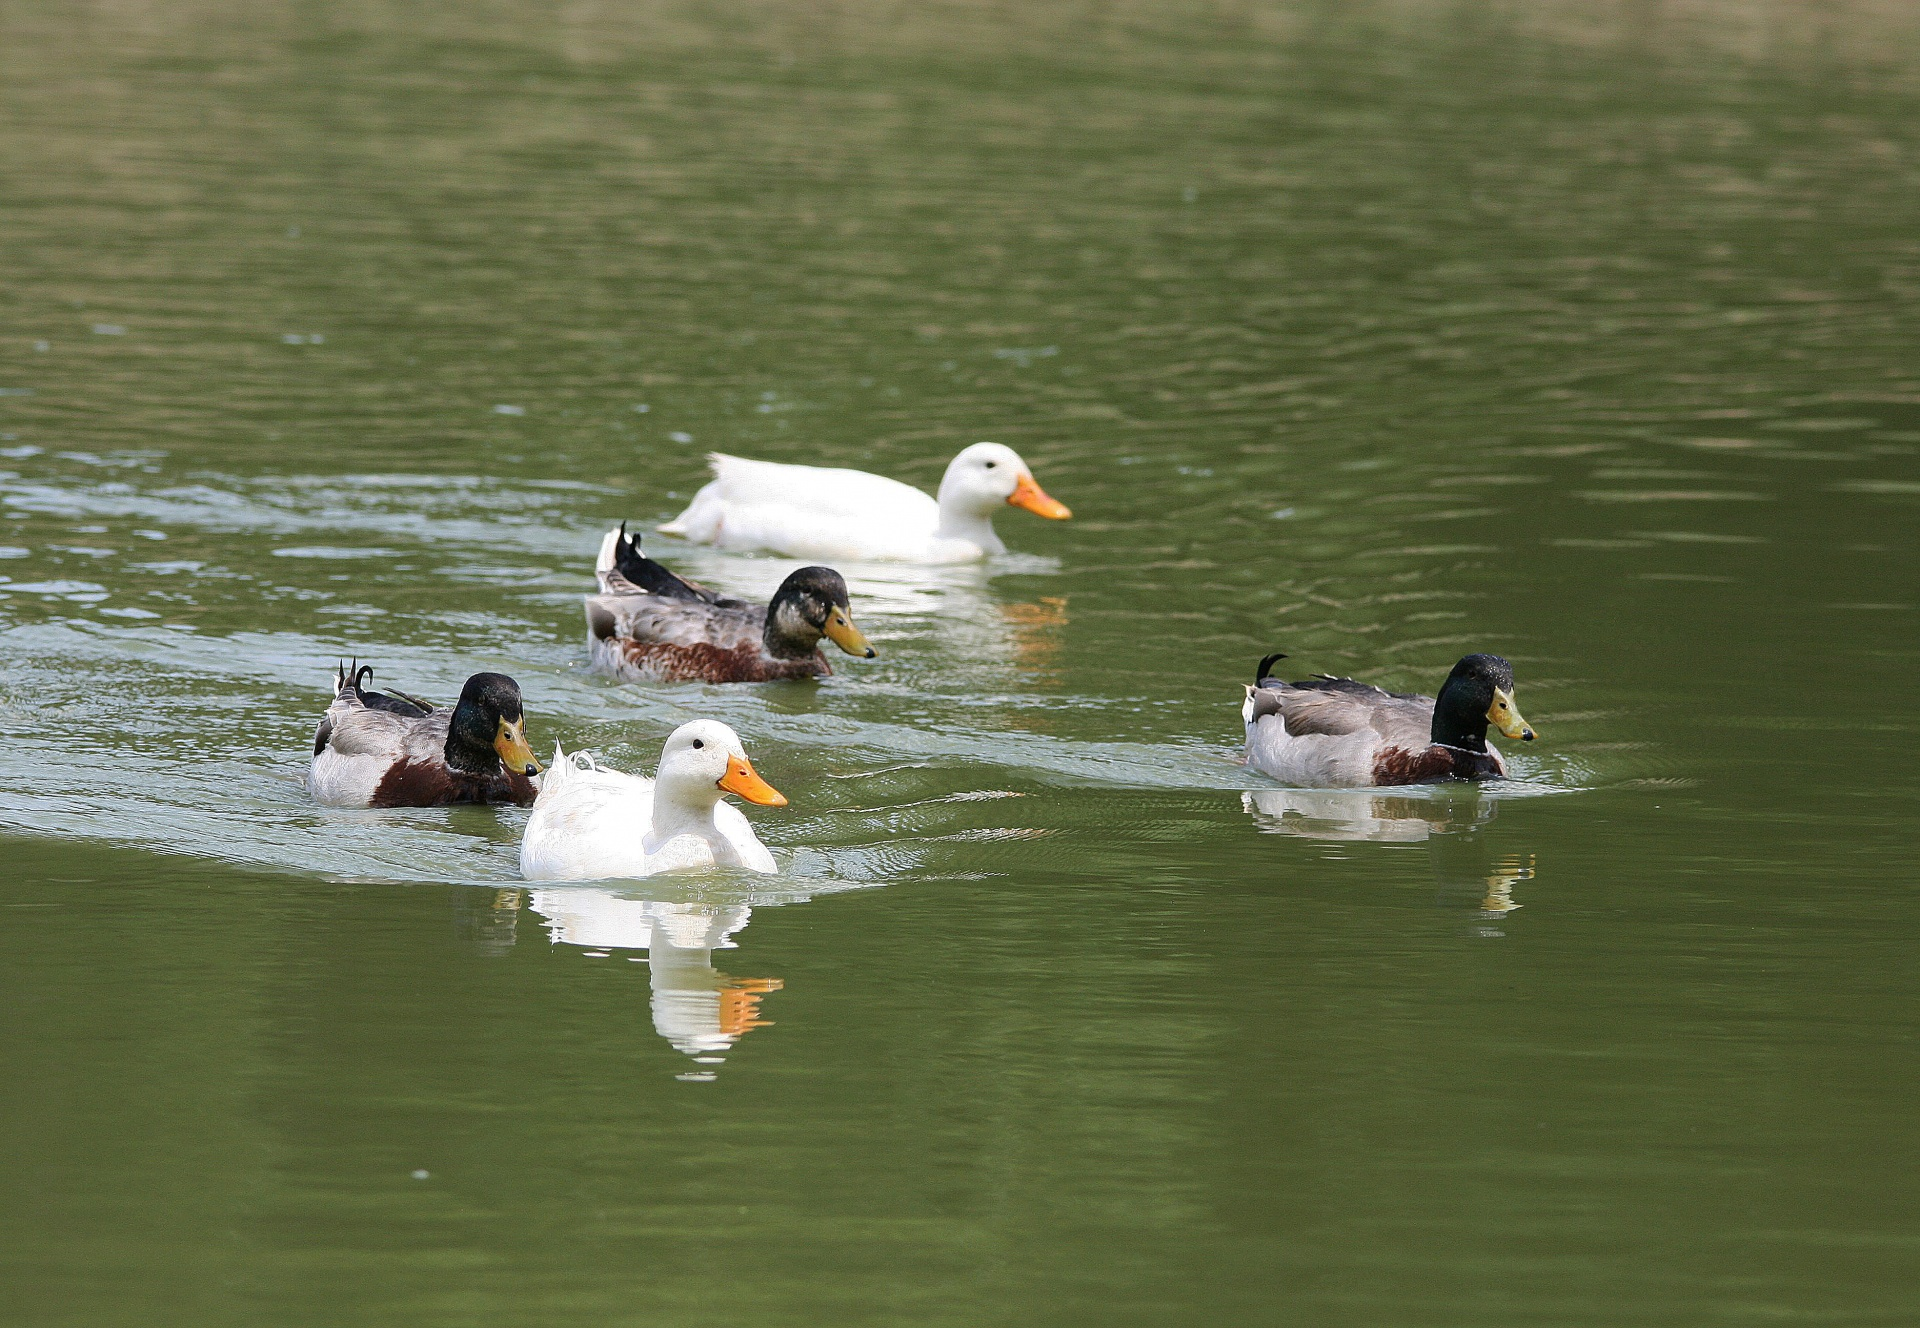
\includegraphics[width=0.8\textwidth]{ducks.png}
    \caption{Enjoy this public-domain picture of ducks I found, as an example.}
    \label{fig:ducks}
\end{figure}
        

Also, see for example Table \ref{tab:cool-table}.

\begin{table}
    \centering
    \begin{tabular}{l|l}
First column & Second column \\
\hline
Yay some text ! & How about some $m\mathbf{A}t\hat{H}$ ?? \\
Should the header text be automatically bold ? & Maybe as an option, we'll see. \\

\end{tabular}

    \caption{This should function as a caption for this table. Does it now ?}
    \label{tab:cool-table}
\end{table}
        
\subsection{New features}

Here is a list of new features allowed by this syntax :
\begin{itemize}
\item 
References ! For this, just surround your label with ** ! For example, see Figure \ref{fig:ducks}. (NB : For this to work, your label must include ":". If it doesn't, add one in front of the label in your reference, like in the proof of Theorem \ref{main-theorem}).

\item 
Labeled equations ! See for example equation (\ref{eq:coffee}).\begin{equation}
	\hat{H}_{\text{int}}=\chi\int _{V}\ket{e} \bra{g} \otimes \hat{a}(\vec{r})d^{3}\vec{r}+\text{h.c.}
\label{eq:coffee}\end{equation}


\item 
Citations ! They work with an external .bib file that has to be named "bibliography.bib". You can cite any paper present in this file by preceding the reference key with an "@". Just like this : \cite{Einstein}.

\item 
Footnotes\footnotemark[1] !

\item 
Additionnal information in a YAML header, which allows you to precise things like title, author(s), date, additionnal LaTeX packages... and more maybe in the future

\end{itemize}
\begin{theorem}[Callouts]

Obsidian callouts can be used to create any LaTeX environment, like theorems and proofs ! In these cases, the relevant packages will be automatically added.\label{main-theorem}
\end{theorem}
\begin{proof}

This is the proof of Theorem \ref{main-theorem}
\end{proof}

\subsection{Options}

I also want to have all equations (display math) to be numbered if I want, even without adding a label manually. Let's see if it works :
\begin{equation}
	E=mc^2
\end{equation}


I had way less ideas for that equation, as you can tell

\footnotetext[1]{ For this, I am copying the syntax from Obsidian.}\n

\end{maincontent}
\printbibliography
\end{document}
